\documentclass[aspectratio=1610,10pt]{beamer}

% \usepackage{algorithmic}
\usepackage[noalgohanging,lined,noend,linesnumbered,onelanguage,portuguese,portuguesekw]{algorithm2e}
\SetAlCapSkip{1.5ex}
% \SetAlFnt{\tiny }
% \SetAlFnt{\scriptsize }
\SetAlFnt{\small}
\setlength{\algomargin}{0em}
\SetInd{.3em}{.5em}
\usetheme[progressbar=frametitle]{metropolis}
\usepackage{appendixnumberbeamer}
\usepackage{booktabs}
\usepackage{xspace}
\usepackage[brazil]{babel}
\usepackage[utf8x]{inputenc}
% \usepackage{lmodern}
\usepackage[alf]{abntex2cite}
% \usepackage{ragged2e}
\usepackage{graphicx}
\usepackage{caption}
\usepackage{subcaption}


\title[]{Uma Implementação Distribuída em Névoa do Algoritmo de Detecção de
Novidade em Fluxos de Dados MINAS}
% \subtitle{Seminários de Metodologia Científica}
\author{Luís Henrique Puhl de Souza\\
Orientador: Prof. Dr. Hermes Senger}
\institute{
Universidade Federal de São Carlos \\
Centro de Ciências Exatas e de Tecnologia \\
Departamento de Computação \\
Programa de Pós-Graduação em Ciência da Computação}
% \date{\today}
\date{05 Julho 2021}
% \titlegraphic{\hfill\includegraphics[height=1.5cm]{logo.pdf}}

\newcommand{\nota}[1]{\hspace*{-0.5cm}\textit{{\color[rgb]{1,0,0}Nota: #1}}}
\newcommand{\minas}{MINAS\xspace}

\begin{document}

\maketitle

\begin{frame}{Índice}
  \setbeamertemplate{section in toc}[sections numbered]
  \tableofcontents[hideallsubsections]
\end{frame}

\section{Introdução}

\begin{frame}[fragile]{Introdução}
  \begin{itemize}%[<+- | alert@+>]
  % Contexto Geral
  \item Crescimento do número de dispositivos IoT e riscos associados;
  \begin{itemize}
    \item[$-$] Heterogeneidade de dispositivos;
    \item[$-$] Falta de atualizações de \emph{software};
    \item[$-$] Exemplo: \emph{Botnet} mirai, infectando cameras e roteadores, gerou
    $620 \ \mathrm{Gb/s}$ \cite{Kambourakis2017}.
  \end{itemize}
  % Contexto Específico
  \item Detecção de intrusão em redes:
  \begin{itemize}
    \item detecção por assinatura \emph{versus} anomalia;
    \item ambiente de névoa e redes IoT.
  \end{itemize}

  % Proposta
  \item Um sistema para detecção de intrusão em Redes IoT implementando em névoa;

  % hipótese
  \item A hipótese do trabalho é que o algoritmo MINAS pode ser distribuído em
  névoa reduzindo a latência e com sem redução na qualidade de classificação.

  \end{itemize}
  % \nota{pode falar:\\
  % - dificuldade de atualização de SW\\
  % - como foi o ataque MIRAI? (só curiosidade)\\
  % - capacidade de autodefesa? mesmo outros computadores não têm...}
\end{frame}


\section{Fundamentos}
\begin{frame}[fragile]{Fundamentos}
\begin{itemize}
  \item Fluxo de Dados e Métodos Detecção de Novidade;
  \item Plataformas de processamento distribuído de fluxos.
  \item Ambientes de computação Distribuída;
\end{itemize}
% \nota{Por que "seria dificil processar de forma centralizado"? [tg] corrigir no discurso}
\end{frame}

\begin{frame}[fragile]{Fundamentos}
  \metroset{block=fill}
  \begin{block}{Definição de Fluxo de Dados}
    
    \vspace{1mm}

    Um fluxo de dados (\textit{Data Stream}) é uma sequência massiva possivelmente
    ilimitada de exemplos multi-dimensionais $x_1, x_2, \dots, x_n, \dots$
    recebidos em instantes associados $t_1, t_2, \dots, t_n, \dots$
  \end{block}

  \metroset{block=transparent}
  \begin{alertblock}{Métodos Detecção de Novidade}
    
    \vspace{1mm}
    Métodos Detecção de Novidade (\emph{Novelty Detection}) lidam com o reconhecimento e
    classificação de exemplos em padrões que diferem de padrões anteriores
    \cite{Gama2010}.
    \begin{itemize}%[<+- | alert@+>]
      
      \item Evolução de Conceito (\emph{Concept Evolution}): surgimento de um conceito durante
      o fluxo;
      
      \item Mudança de Conceito (\emph{Concept Drift}, deriva ou desvio): modificação da
      distribuição de um padrão conhecido. A modificação pode ser repentina,
      incremental ou recorrente;
      
      \item Ruído e \emph{Outliers}: que não pertencem a um conceito ou
      pertencem a um conceito porém estão fora da distribuição conhecida.
      
    \end{itemize}
  \end{alertblock}
% \nota{Poderia explicar melhor a evolução de modelos, "concept drift"
% (precisa estudar um pouco + a teoria).}
\end{frame}

\begin{frame}[fragile]{Fundamentos}
\begin{alertblock}{Algoritmo MINAS e suas estratégias}
  \vspace{5mm}
  \begin{itemize}%[<+- | alert@+>]
    \item Modelo de aprendizado \emph{Offline-Online};
    \item Transformação dos dados analisados para o espaço $\mathbb{R}^d$;
    \item Modelo de classificação com \emph{Clusters};
    \item Função de classificação baseada em distância euclideana;
    \item Algoritmo de agrupamento para identificação de novos padrões;
    \item Classificação de novos padrões entre recorrência, extensão e novidade;
  \end{itemize}
\end{alertblock}
% \nota{MINAS: Use figura!\\pseudocodigo?}
\end{frame}

\begin{frame}[fragile]{Fundamentos}
\begin{figure}[ht]
  \centering
  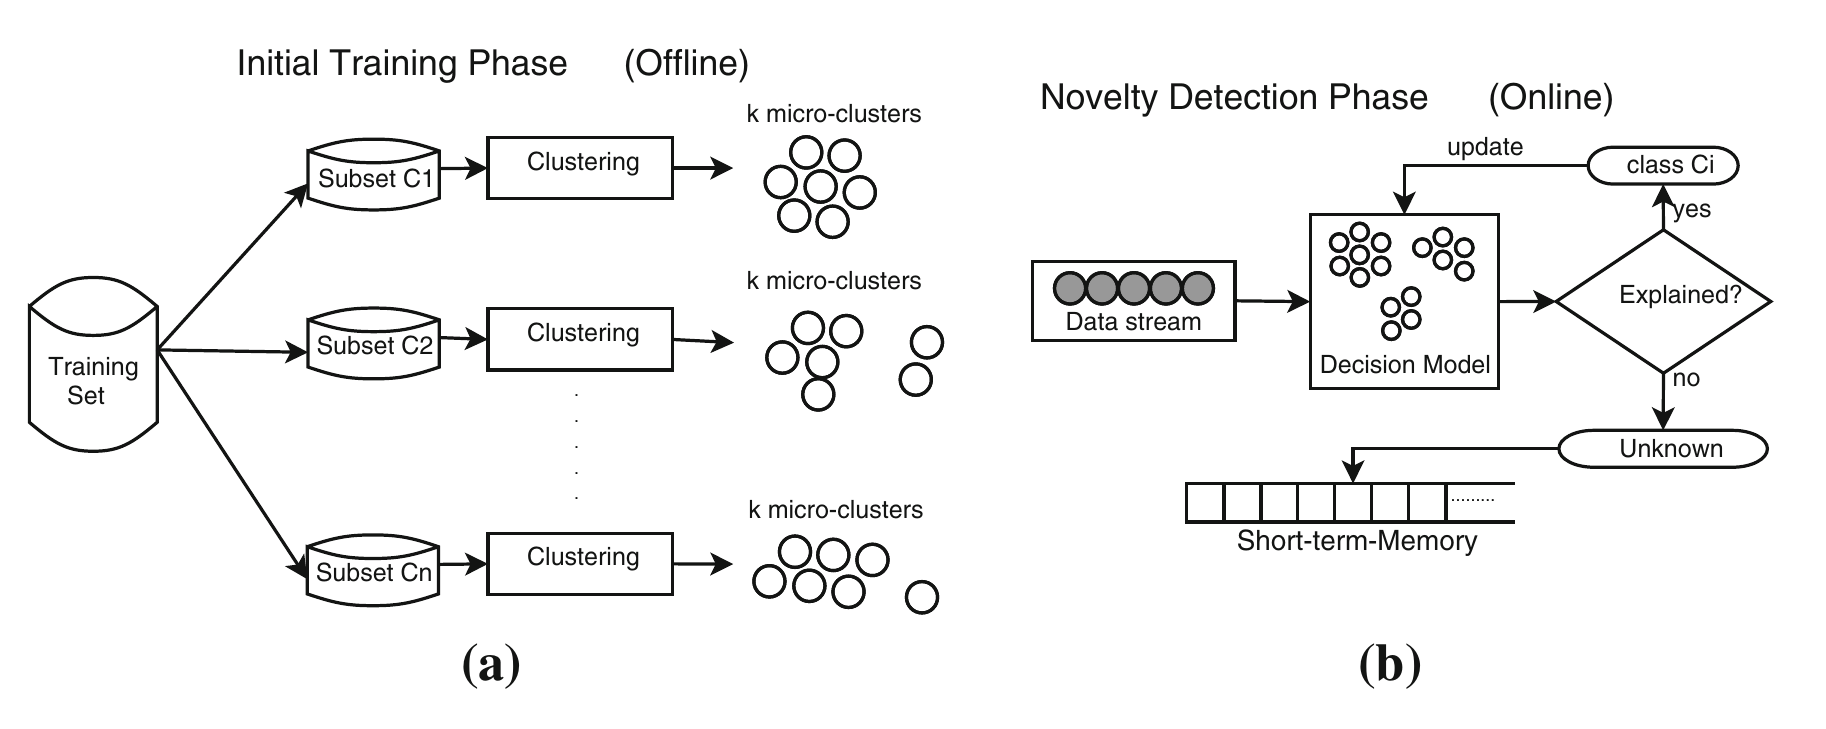
\includegraphics[width=\textwidth]{figuras/FariaMinas2015-fases.png}
  \caption{Visão geral do algoritmo MINAS com fases \emph{Offline} (a) e 
  \emph{Online} (b). \textbf{Fonte:} \citeonline{Faria2016minas}.}
  \label{fig:minas}
\end{figure}
% \nota{Explique o desenho! o que significa cada objeto da figura? explique na figura.}
\end{frame}

\begin{frame}
\begin{algorithm}[H]
  \SetKwFunction{nearestCluster}{clusterMaisPróximo}
  \SetKwFunction{NoveltyDetection}{DetecçãoNovidade}
  \SetKwFunction{handleModelSleep}{moveModeloAntigo}
  \SetKwFunction{removeOldSamples}{removeExemplosAntigos}
  % 
  \SetKwProg{Function}{Função}{:}{}
  \SetKwData{cleaningWindow}{janelaLimpeza}
  \SetKwData{noveltyDetectionTrigger}{gatilhoDetecçãoNov}
  \SetKwFunction{MinasOnline}{MinasOnline}
  % 
  \Function{\MinasOnline{Modelo, fluxoEntrada, fluxoSaída, \cleaningWindow, \noveltyDetectionTrigger}}{
    Desconhecidos $\leftarrow$ $\emptyset$; ModeloAntigo $\leftarrow$ $\emptyset$; últimaLimpeza $\leftarrow 0$; proximaNovidade $\leftarrow 0$\;
    \ForEach{ {$exemplo_{i}$} $\in$ fluxoEntrada }{
      % exemplo.rótulo $\leftarrow$ unknown\;
      % (distância, cluster) $\leftarrow$ \nearestCluster(exemplo, Modelo)\;
      maisPróximo $\leftarrow$ \nearestCluster(exemplo, Modelo)\;
      \eIf{maisPróximo.distância $<$ maisPróximo.cluster.raio}{
        exemplo.rótulo $\leftarrow$ maisPróximo.cluster.rótulo\;
        maisPróximo.cluster.últimoUso $ \leftarrow i$\;
      }
      {
        exemplo.rótulo $\leftarrow$ ``desconhecido''\;
        Desconhecidos $\leftarrow$ Desconhecidos $\cup$ exemplo\;
        \If{$|\;Desconhecidos\;| \geq$ \noveltyDetectionTrigger}{
          Modelo $\leftarrow$ Modelo $\cup$ \NoveltyDetection(Modelo $\cup$ ModeloAntigo, *Desconhecidos)\;
        }
        \If{ $ i > $ ( últimaLimpeza $ + $ \cleaningWindow )}{
          Modelo $\leftarrow$ \handleModelSleep(Modelo, *ModeloAntigo, últimaLimpeza)\;
          Desconhecidos $\leftarrow$ \removeOldSamples(Desconhecidos, últimaLimpeza)\;
          últimaLimpeza $ \leftarrow i $\;
        }
      }
      fluxoSaída.adicione(exemplo)\;
    }
  }
  \caption{Interpretação do algoritmo \minas \emph{online} \cite{Faria2016minas}.}
\label{alg:minas-main}
\end{algorithm}
\end{frame}

\begin{frame}[fragile]{Fundamentos}
  \begin{alertblock}{Plataformas de processamento distribuído}
    \vspace{5mm}
    \begin{columns}[T,onlytextwidth]
        \column{0.5\textwidth}
        \begin{itemize}%[<+- | alert@+>]
          \item Arquiteturas \emph{Lambda} e \emph{Kappa};
          \item Mineração de Dados:
          \begin{itemize}
            \item \emph{MapReduce} e \emph{Apache Hadoop};
            \item \emph{Apache Spark} com \emph{Resilient Distributed Dataset - RDD};
          \end{itemize}
          \item Mineração de Fluxo de Dados:
          \begin{itemize}
            \item \emph{Apache Spark Streaming} com estratégia de \emph{micro-batching};
            \item \emph{Apache Storm};
            \item \emph{Apache Flink};
          \end{itemize}
          \item Não especializadas em fluxo de dados:
          \begin{itemize}
            \item Não-plataforma (construção dos mecanismos de envio e recebimento);
            \item Interface de Troca de Mensagens - MPI;
          \end{itemize}
        \end{itemize}
        \column{0.05\textwidth}
        \column{0.45\textwidth}
        \begin{figure}
            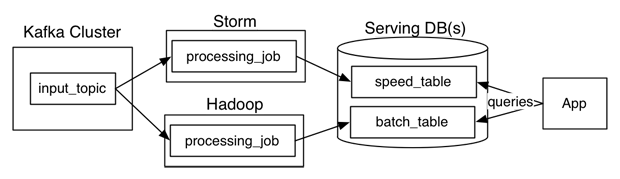
\includegraphics[width=0.9\textwidth]{figuras/lambda.png}
            \caption{Arquitetura Lambda com Kafka, Storm, Hadoop, SGBD tradicional e aplicação consumidora.}
        \end{figure}
        \begin{figure}
            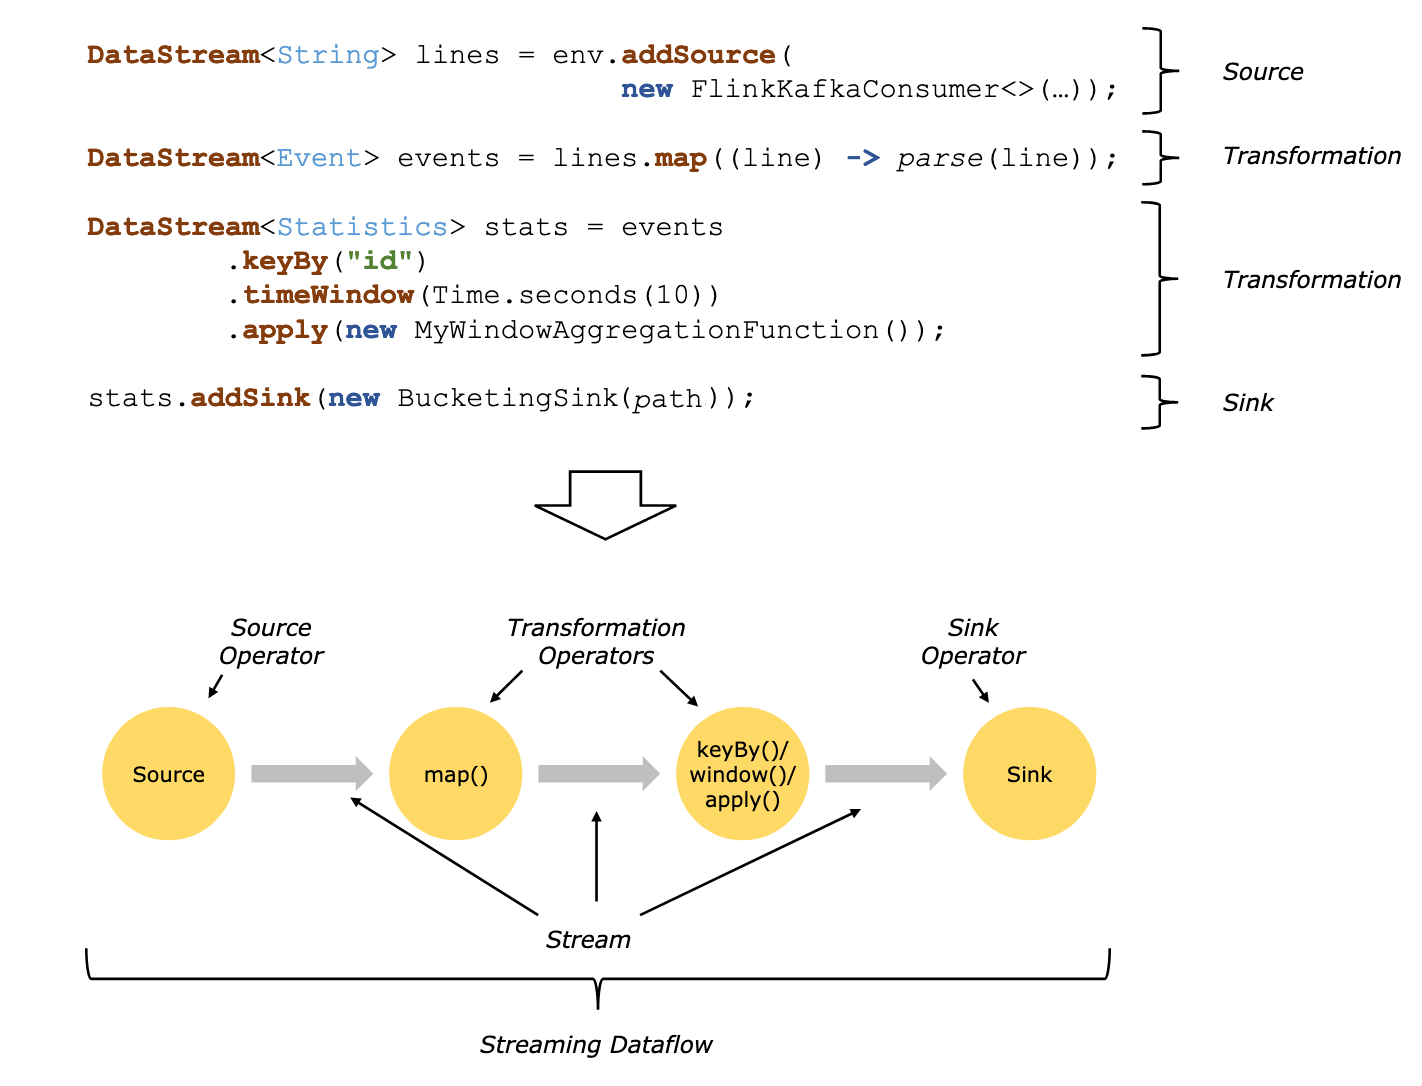
\includegraphics[width=0.9\textwidth, trim={0 0 10cm 20cm},clip]{figuras/dataflow-code-flink.png}
            \caption{Arquitetura Apache Flink.}
        \end{figure}
    \end{columns}
  \end{alertblock}

  % \nota{Faltou definir antes o que é processamento de fluxo.\\
  % \textbf{fluxo vs lote} deixar mais claro a diferença}

  % \nota{O slide fala de plataformas, mas vc falou de kappa e lambda
  % que não deveria falar neste slide}

  % \nota{Muita fala p/ esse slide (ficou explicando cada fundamento).
  % Deveria quebrar o slide em 3 ou 4 slides ao menos.}
\end{frame}

\begin{frame}[fragile]{Fundamentos - MPI}
  \begin{itemize}%[<+- | alert@+>]
    \item Localidade de dados;
    \begin{itemize}
      \item Menor número de \emph{page-faults} mantendo o Modelo em cache;
    \end{itemize}
    \item Memória distribuída e troca de mensagens;
    \item Padrão MPI - \emph{Message Passing Interface};
    \begin{itemize}
      \item Bibliotecas bem estabelecidas;
      \item Pares de operações \emph{send/receive}, entre outras operações;
      \item Execução gerenciada (\emph{Runtime Environment}, \texttt{mpirun});
    \end{itemize}
    \item Técnica SPMD - \emph{Single Program Multiple Data};
    \begin{itemize}
      \item Construção simplificada;
    \end{itemize}
  \end{itemize}
\end{frame}

\begin{frame}[fragile]{Fundamentos}
\begin{alertblock}{Ambientes de computação Distribuída}
\begin{itemize}
  \item Computação em Nuvem (\emph{Cloud Computing}) é um modelo que permite
  acesso conveniente a recursos computacionais compartilhados \cite{NIST2011}
  \begin{columns}[T,onlytextwidth]
    \column{0.5\textwidth}
    \begin{itemize}
      \item \textbf{Características Essenciais:}
      \begin{itemize}
        \item Auto-serviço sob demanda,
        \item Amplo acesso à rede,
        \item Agrupamento de recursos,
        \item Rápida elasticidade,
        \item Serviço mensurado;
      \end{itemize}
    \end{itemize}
    \column{0.5\textwidth}
    \begin{itemize}
      % \item \textbf{Modelo de Serviço:} \emph{Software} (SaaS), Plataforma (PaaS), Infraestrutura (IaaS);
      % \item \textbf{Implementações:} privada, comunitária, pública, híbrida.
      \item \textbf{Modelo de Serviço:}
      \begin{itemize}
        \item \emph{Software} (SaaS),
        \item Plataforma (PaaS),
        \item Infraestrutura (IaaS),
      \end{itemize}
      \item \textbf{Implementações:}
      \begin{itemize}
        \item Nuvem privada,
        \item Nuvem comunitária,
        \item Nuvem pública,
        \item Nuvem híbrida.
      \end{itemize}
    \end{itemize}
  \end{columns}
\end{itemize}
\end{alertblock}
% \nota{Separar os items em bullets (sub-bullets)}
\end{frame}

\begin{frame}[fragile]{Fundamentos}
\begin{alertblock}{Ambientes de computação Distribuída}
\begin{itemize}
  \item Computação de Borda (\emph{Edge Computing}):
  \\ Refere-se a qualquer recurso computacional ou de rede entre os dispositivos
  de borda e centro de dados hospedados em nuvem \cite{Shi2016}.

  \item Computação em Névoa (\emph{Fog Computing})
  
  % \cite{Bonomi2012,dastjerdi2016}
  
  % A horizontal, system-level architecture that distributes
  % computing, storage, control and networking functions closer to
  % the users along a cloud-to-thing continuum.
  
  Uma arquitetura horizontal a nível de sistema que distribui funções de
  computação, armazenamento, controle e rede próximos aos usuários no espaço
  contínuo nuvem-coisa \cite{IEEECommunicationsSociety2018}.
  \textbf{Características:}
  % \hspace{0.2\textwidth}
  \begin{columns}
    \column{0.15\textwidth}
    \column{0.3\textwidth}
    \begin{itemize}
      \item Mobilidade,
      \item Heterogeneidade,
      \item Baixa Latência,
      \item Distribuição geográfica,
    \end{itemize}
    \column{0.4\textwidth}
    \begin{itemize}
      \item Alto número de nós,
      \item Interoperabilidade e federação,
      \item Uso de fluxo de dados e aplicações em tempo real.
    \end{itemize}
    \column{0.15\textwidth}
  \end{columns}
  % \begin{block}{Características:}
  % \end{block}
\end{itemize}
\end{alertblock}
\end{frame}

% ------------------------------------------------------------------------------

\section{Estado da Arte e Trabalhos Relacionados}
\newcommand{\arch}{IDSA-IoT\xspace}

\begin{frame}[fragile]{Estado da Arte e Trabalhos Relacionados}
\begin{alertblock}{Sistemas de detecção de intrusão em redes}
  \begin{itemize}
    \item Ferramenta BigFlow \cite{Viegas2019}:
    \begin{itemize}
      % \nota{% OK, isso é trabalho relacionado!\\
      % Dissecar melhor [bigflow, catraca, idsa-iot]\\
      % passar mais rápido, detalhar nos próximos.}
      % \nota{BigFlow usa stream mining?\\
      % - qual é a grande contribuição?\\
      % - qual é a limitação?}
      \item[$\boldsymbol{+}$] Integração da extração dos descritores de fluxo à emissão de alarmes;
      \item[$\boldsymbol{+}$] Capacidade de tratamento de grandes volumes;
      \item[$\boldsymbol{-}$] Atualização semanal com avaliação de um especialista;
      \item[$\boldsymbol{-}$] Execução somente em nuvem.
    \end{itemize}
    \item Ferramenta CATRACA \cite{Lopez2018,Sanz2018}:
    \begin{itemize}
      % \nota{catraca: contribuição? limitação?}
      \item[$\boldsymbol{+}$] Divisão em camadas alocadas em nuvem e névoa;
      \item[$\boldsymbol{+}$] Modelo de decisão baseado em árvore de decisão;
      \item[$\boldsymbol{-}$] Extração dos descritores de fluxo é feita em
      névoa, classificação e detecção é feita em nuvem.
    \end{itemize}
    \item Arquitetura \arch \cite{Cassales2019a}:
    \begin{itemize}
      \item[$+$] Avaliação do algoritmo MINAS, ECSMiner e AnyNovel;
      \item[$+$] Distribuição das tarefas em nuvem e névoa focada em IoT;
      \item[$-$] Implementação e detalhamento da arquitetura em aberto.
    \end{itemize}
  \end{itemize}
\end{alertblock}
\end{frame}

\begin{frame}[fragile]{Estado da Arte e Trabalhos Relacionados}
\begin{figure}[ht]
  \centering
  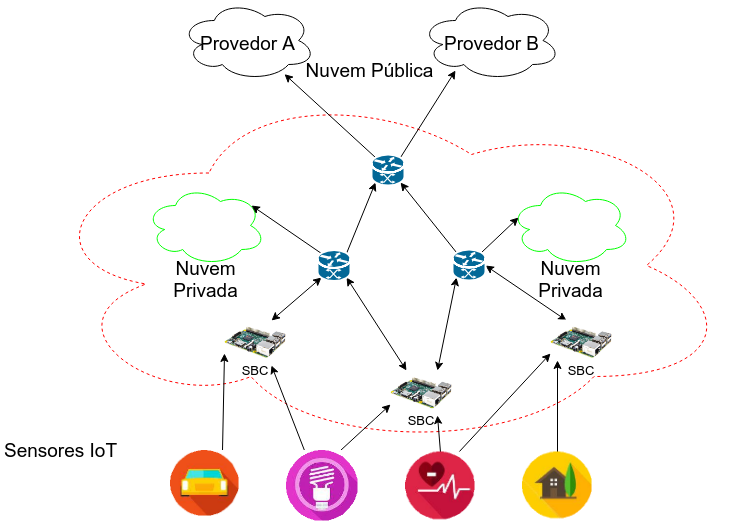
\includegraphics[width=0.48\textwidth]{figuras/idsa-iot-quali-000.png}
  \hfill
  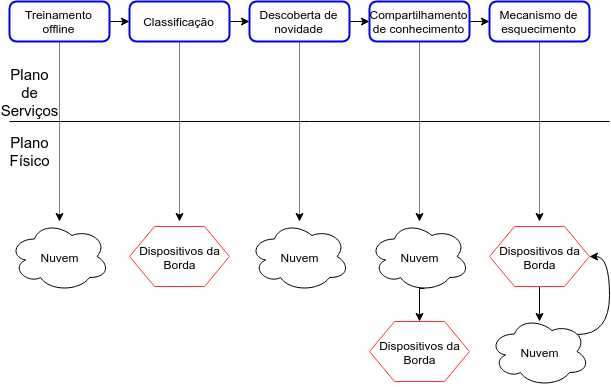
\includegraphics[width=0.48\textwidth]{figuras/idsa-iot-quali-004.png}
  \caption{Distribuição de serviços da arquitetura \arch. \textbf{Fonte:} \citeonline{Cassales2019a}.}
  \label{fig:ids-iot}
\end{figure}
\end{frame}

\newcommand{\mfog}{sistema M-FOG\xspace}

\section{Proposta}

\begin{frame}[fragile]{Proposta}
  \metroset{block=fill}
  \begin{block}{Pergunta de Pesquisa}
    \begin{itemize}
      \item É viável implementar a arquitetura \arch?
      \item É viável paralelizar e distribuir o algoritmo MINAS?
      \item Quais são os efeitos na qualidade de classificação paralelizar e
      distribuir o algoritmo MINAS?
      
      % Proposta
      \item Um sistema para detecção de intrusão em Redes IoT implementando em névoa;

      % hipótese
      \item A hipótese do trabalho é que o algoritmo MINAS pode ser distribuído em
      névoa reduzindo a latência e com sem redução na qualidade de classificação.

      % \nota{pode falar:\\
      % - dificuldade de atualização de SW\\
      % - como foi o ataque MIRAI? (só curiosidade)\\
      % - capacidade de autodefesa? mesmo outros computadores não têm...}
    \end{itemize}
  \end{block}
\end{frame}

\begin{frame}[fragile]{Proposta}
  \metroset{block=fill}
  \begin{block}{Proposta da Pesquisa}
    \begin{itemize}
      
      \item Implementar a distribuição do algoritmo MINAS em nuvem e névoa
      conforme arquitetura \arch;
      
      \item Paralelizar o método de classificação do algoritmo MINAS.
    \end{itemize}
  \end{block}

  \metroset{block=transparent}
  \begin{alertblock}{Métodologia}
    \begin{itemize}%[<+- | alert@+>]
      \item Plataforma de processamento distribuído;
      \item Estratégias de implementação da arquitetura \arch;
      \item Experimentação com a distribuição do algoritmo MINAS em ambientes;
      \item Métricas de qualidade de classificação para validação da implementação;
      \item Métricas de escalabilidade.
    \end{itemize}
  \end{alertblock}
  % \nota{Proposta\\
  % - poderia fazer algumas "perguntas" antes de fazer a sua proposta\\
  % => quais perguntas? (voce precisa saber quais)}
\end{frame}


\begin{frame}[fragile]{Proposta}

  O \mfog é dividido em 5 módulos subdivididos em 2 grupos.
  
  \begin{alertblock}{Módulos principais implementam o algoritmo MINAS}
    \begin{itemize}
      \item TODO;
    \end{itemize}
  \end{alertblock}

\end{frame}

\begin{frame}
  \begin{figure}[h]
    \centering
    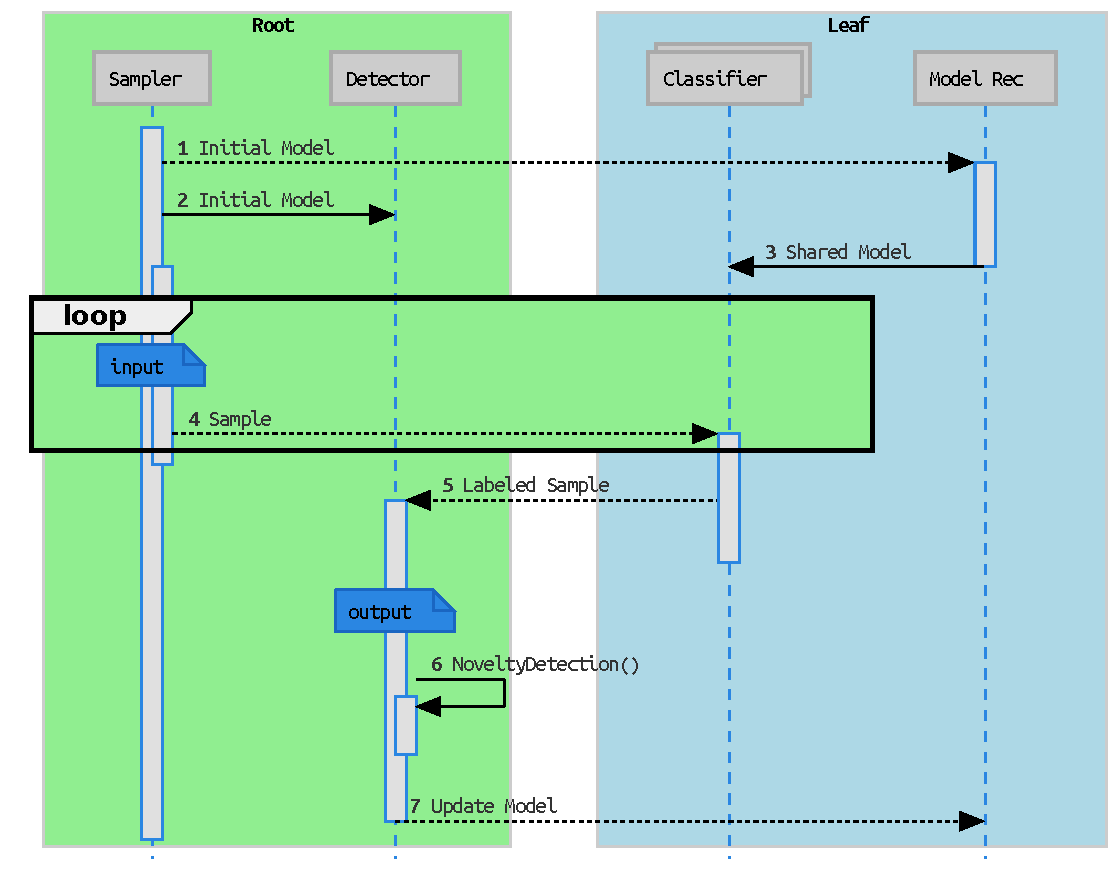
\includegraphics[width=0.88\textwidth,page=1]{figures/lifecycle-uml-svg.pdf}
    \caption{Arquitetura e fluxos de dados do \mfog.}
    \label{fig:arch}
  \end{figure}
\end{frame}

\section{Resultados}
\begin{frame}[fragile]{Resultados}

  \begin{alertblock}{Primeira Implementação com \emph{Python} e \emph{Apache Kafka}}
    \begin{itemize}%[<+- | alert@+>]
      \item \emph{Python} é acessível e fornece bibliotecas diversas;
      \item \emph{Apache Kafka} é um sistema de mensagens distribuído;
      \begin{itemize}
        \item Interface de programação com cliente produtor e consumidor;
        \item Mensagens organizadas em tópicos que são distribuídos em partições;
      \end{itemize}
      \item A hipótese de que a carga seria distribuída entre os consumidores,
      uma vez que o consumidor pode selecionar uma partição para leitura;
      \item Em experimento com um produtor, 8 partições e 8 consumidores,
      observou-se que um consumidor processava a maior parte das mensagens,
      poucos consumidores recebiam algumas mensagens e a maioria dos consumidores
      não recebia mensagem alguma.
    \end{itemize}
  \end{alertblock}
% \nota{\textsc{cuidado,} o fato de vc não ter conseguido não significa que não é possível\\
% concluir que "o sistema não escala ..." (pode citar, só tome cuidado com a conclusão tirada)}
\end{frame}

\begin{frame}[fragile]{Resultados}
  \begin{alertblock}{Segunda Implementação com \emph{Apache Flink}}
    \begin{itemize}%[<+- | alert@+>]
      \item Implementação escrita em Scala ou Java;
      \item Processamento de fluxos \emph{Stateful};
      \item Falta de bibliotecas que distribuam algoritmos base como \emph{K-means};
      \item Gerenciador de trabalhos (\emph{job manager}) e gerenciador de
      tarefas (\emph{job manager}) ocupam mais de $1\;GB$ em execuções
      consecutivas, portanto não é confiável para dispositivos pequenos.
    \end{itemize}
  \end{alertblock}
% \nota{métricas: Tem a fórmula? expressão?}

% \nota{"Avaliação do fluxo de saída do classificador" isto é uma métrica?}

% \nota{Incluir CR}
\end{frame}

\begin{frame}[fragile]{Resultados}
  \begin{alertblock}{Métricas e Ambientes}
    \begin{itemize}
      \item Métricas de qualidade de classificação:
      \begin{itemize}
        \item Avaliação do fluxo de saída do classificador;
        \item Uso de uma matriz de confusão ou erro;
        \item Taxa de desconhecidos;
        \item Macro F-score;
      \end{itemize}
    \end{itemize}
  \end{alertblock}

  \begin{columns}[T,onlytextwidth]
    \column{0.5\textwidth}
  %   \begin{equation*}
  %     \mathbf{E}_n = \begin{pmatrix}
  %       e_{1,1} & e_{1,2} & \cdots & e_{1,J} \\
  %       e_{2,1} & e_{2,2} & \cdots & e_{2,J} \\
  %       \vdots  & \vdots  & \ddots & \vdots  \\
  %       e_{M,1} & e_{M,2} & \cdots & e_{M,J} 
  %     \end{pmatrix}
  %   \end{equation*}
    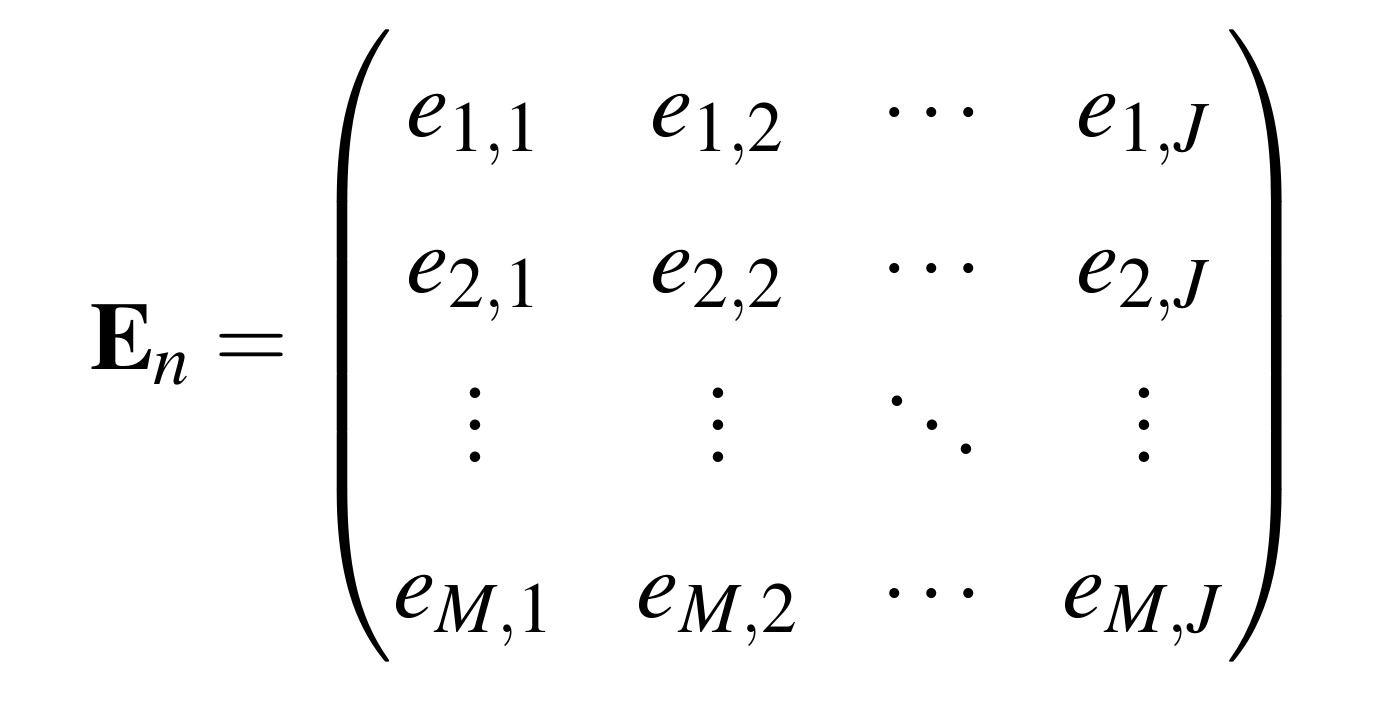
\includegraphics[width=0.9\textwidth]{figuras/eq-matrix.png}
    \column{0.5\textwidth}
    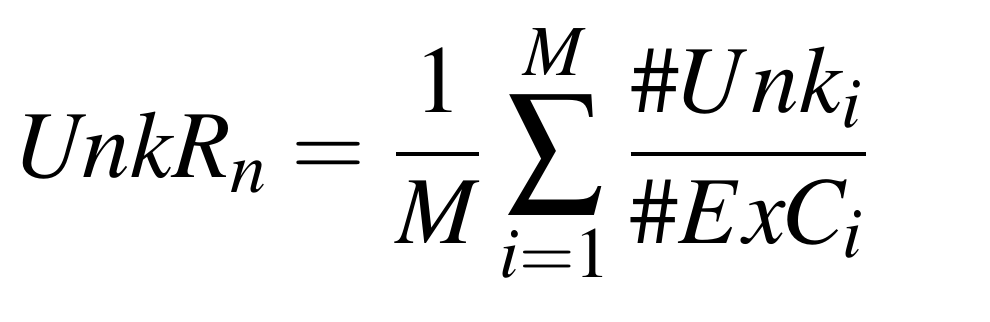
\includegraphics[width=0.9\textwidth]{figuras/eq-unk.png}
    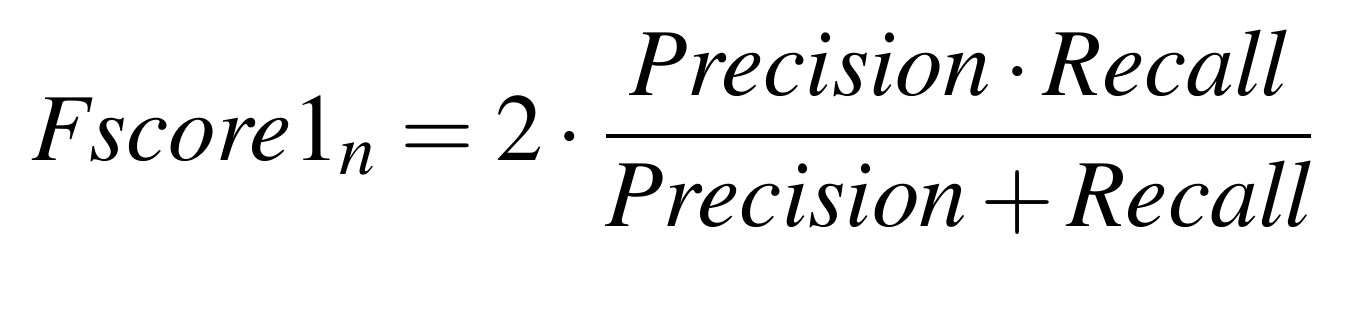
\includegraphics[width=0.9\textwidth]{figuras/eq-fscore1.png}
  %   \begin{equation*}
  %       \mathit{UnkR}_n      = \frac{1}{M} \sum_{i=1}^{M} \frac{\#Unk_i}{\#ExC_i} \\
  %       \mathit{Fscore}1_n   = 2 \cdot \frac{
  %         \mathit{Precision} \cdot \mathit{Recall}
  %         }{
  %           \mathit{Precision} +\mathit{Recall}
  %         }
  %   \end{equation*}
  \end{columns}
\end{frame}

\begin{frame}[fragile]{Resultados}
  \begin{alertblock}{Métricas e Ambientes}
    \begin{itemize}
      \item Métricas de escalabilidade:
      \begin{itemize}
        \item Número e tipo de processadores;
        \item Uso de memória;
        \item Tempo de processamento;
        \item Taxa de eventos;
        \item Latência entre a produção e classificação.
      \end{itemize}
      \item Ambientes de teste:
      \begin{itemize}
        \item Computador Pessoal (para desenvolvimento);
        \item Nevoa composta de SBC (\emph{Sigle Board Computer}) ARM 4 núcleos;
        \item Conjunto de dados para IDS, Kyoto 2006+, segmento dezembro de 2015
        como estabelecido por \citeonline{Cassales2019a}.
      \end{itemize}
    \end{itemize}
  \end{alertblock}
\end{frame}

\newcommand{\expA}{\textit{a-Referência}\xspace}
\newcommand{\expB}{\textit{b-Sequencial}\xspace}
\newcommand{\expC}{\textit{c-Paralelo}\xspace}
\newcommand{\expD}{\textit{d-Distribuído}\xspace}
\begin{frame}[fragile]{Resultados}
  \begin{alertblock}{Experimentos}
    \begin{table}[htb]
      \centering
      \begin{tabular}{p{0.17\textwidth}|p{0.27\textwidth}|p{0.47\textwidth}}
      \textbf{Experimento} & \textbf{Programa}                 & \textbf{Características} \\\hline
      \expA                & \minas referência 2013            & Raio é a distância máxima. \\\hline
      \expB                & \minas sequencial para validação  & 
        Raio é o desvio padrão das distâncias;
        Modelo único;
        Remoção de desconhecidos mais agressivo. \\\hline
      \expC                & \mfog 1 nó, 4 processadores       & 
        Classificadores paralelos;
        Detecção de novidade assíncrona. \\\hline
      \expD                & \mfog 3 nós, 12 processadores     &
        Mais processadores;
        Comunicação em rede.
      \end{tabular}
      \caption{Listagem dos principais experimentos.}
    \end{table}
  \end{alertblock}
\end{frame}

\begin{frame}[fragile]{Resultados}
  \begin{figure}
    \begin{subfigure}{0.49\textwidth}
      \centering
      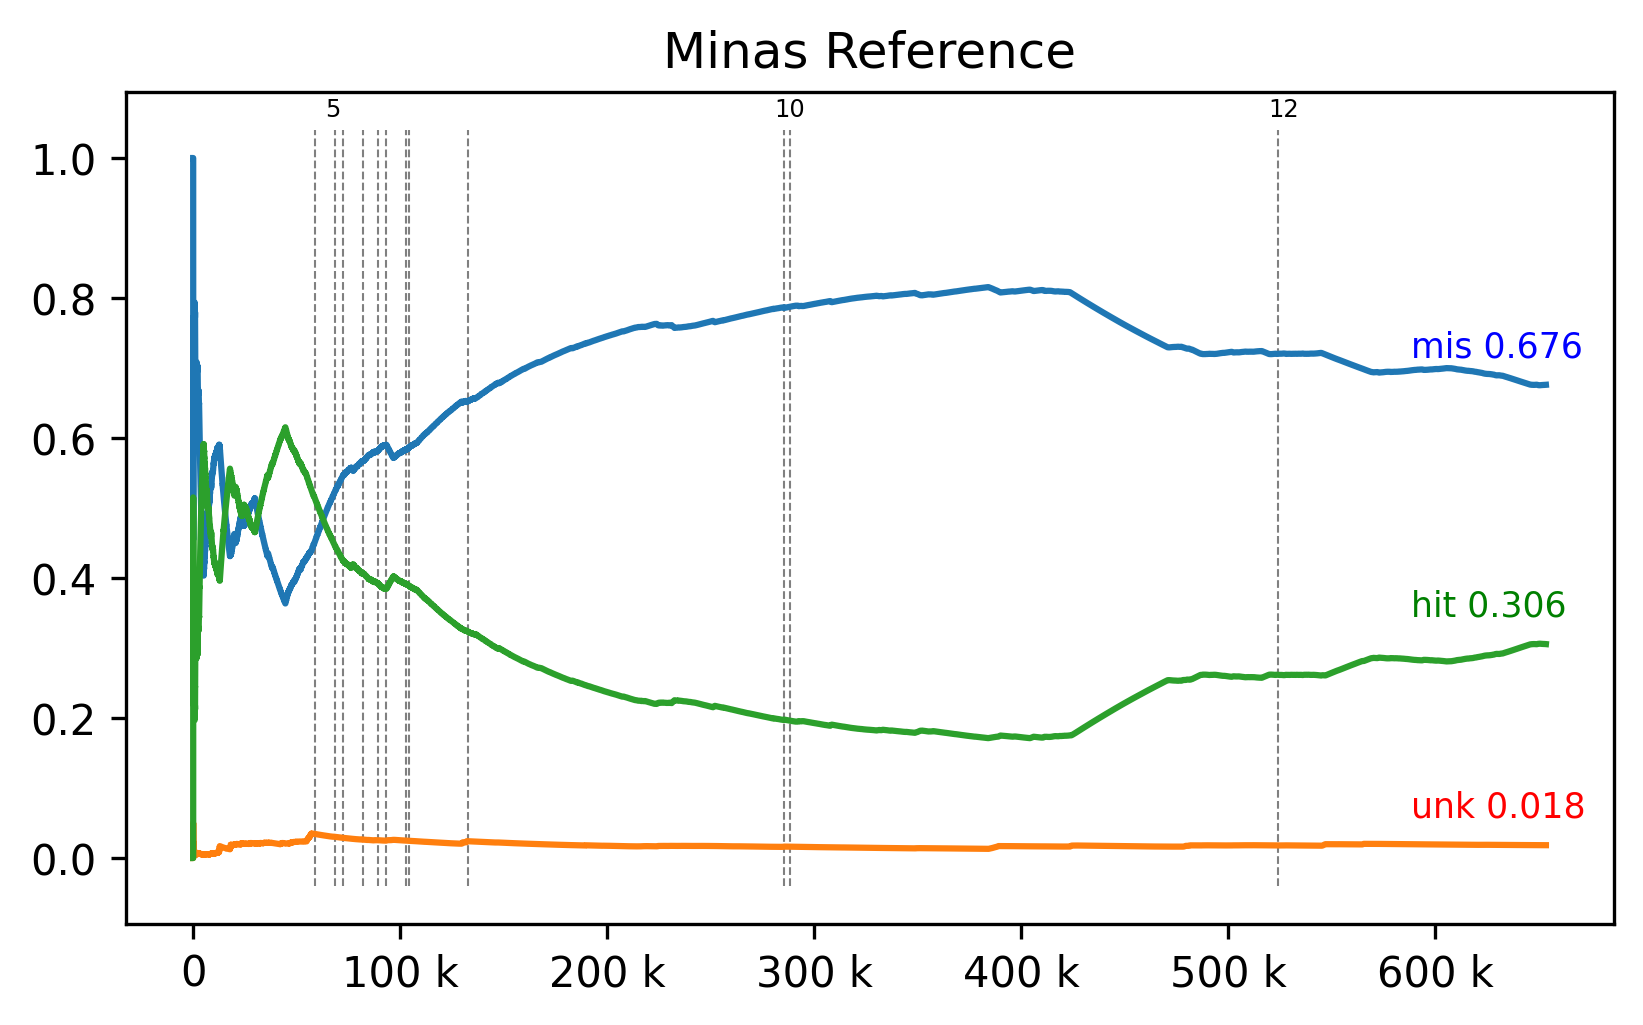
\includegraphics[width=1\linewidth]{experiments/revised-java-log.png}
      \caption{Experimento \expA, implementação de referência do algoritmo \minas.}
      \label{fig:validation-java}
    \end{subfigure}
    \hfill
    \begin{subfigure}{0.49\textwidth}
      \centering
      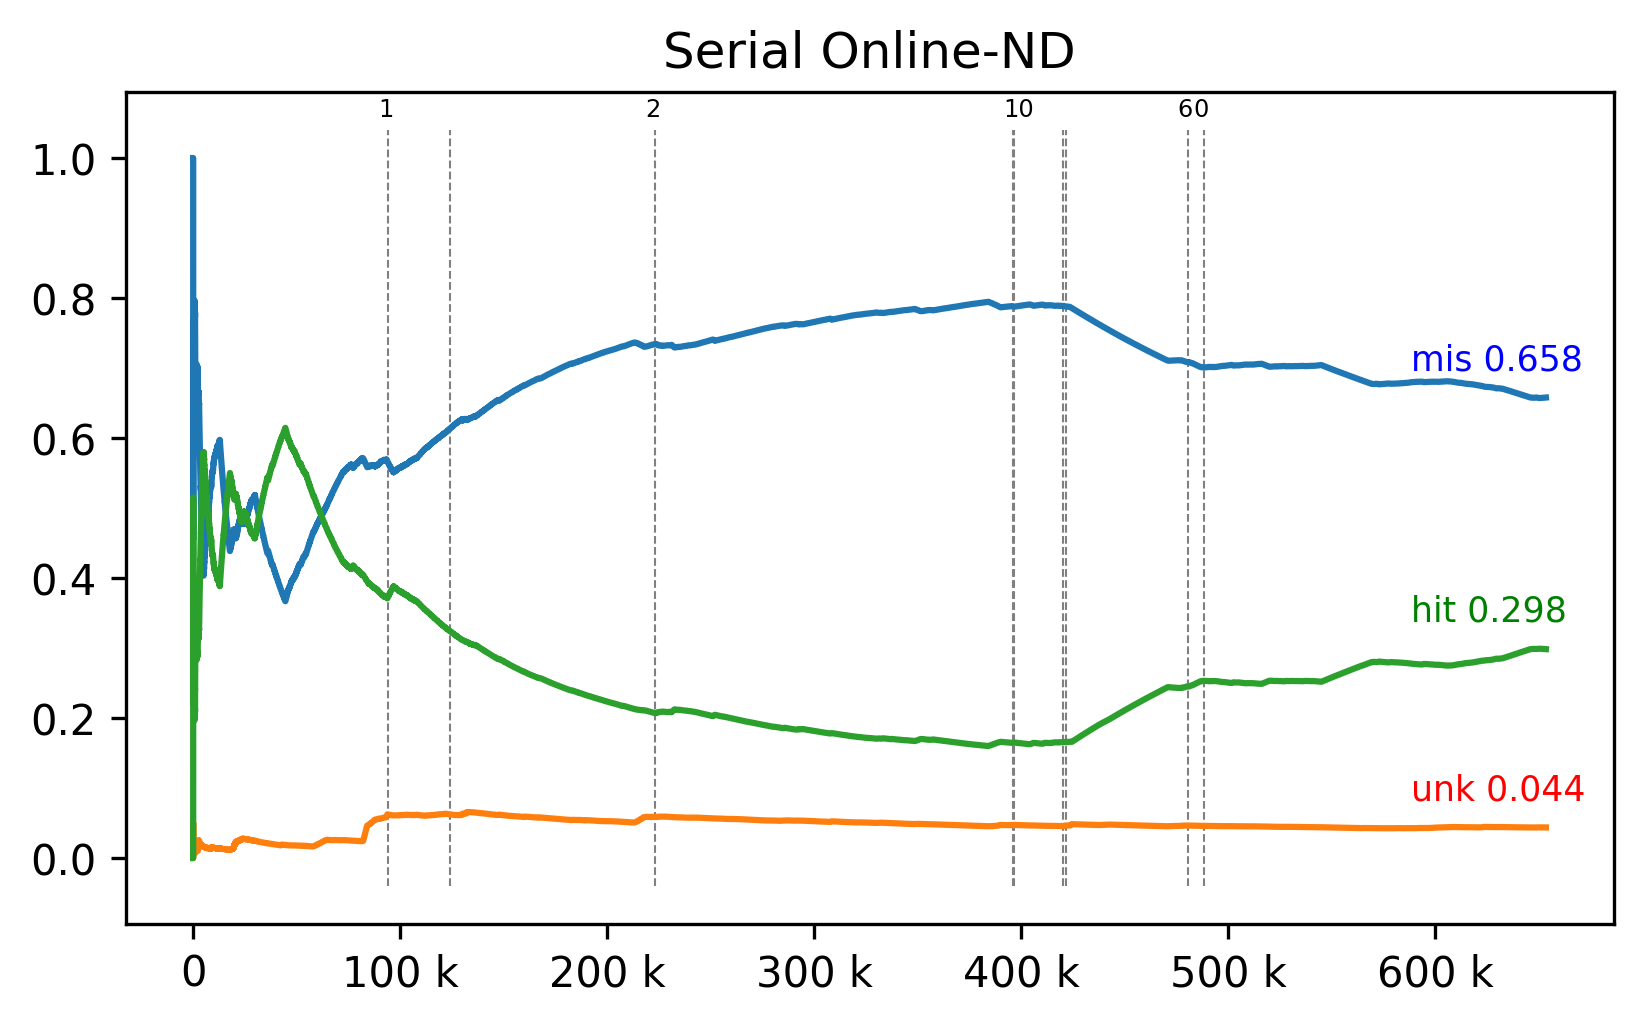
\includegraphics[width=1\linewidth]{experiments/online-nd-log.png}
      \caption{Experimento \expB, \mfog sequencial.}
      \label{fig:validation-serial}
    \end{subfigure}
    \caption{Visualização de fluxo do conjunto \emph{Kyoto} Dez. 2015.}
  \end{figure}
\end{frame}

\begin{frame}[fragile]{Resultados}
  \begin{figure}
    \begin{subfigure}{0.49\textwidth}
      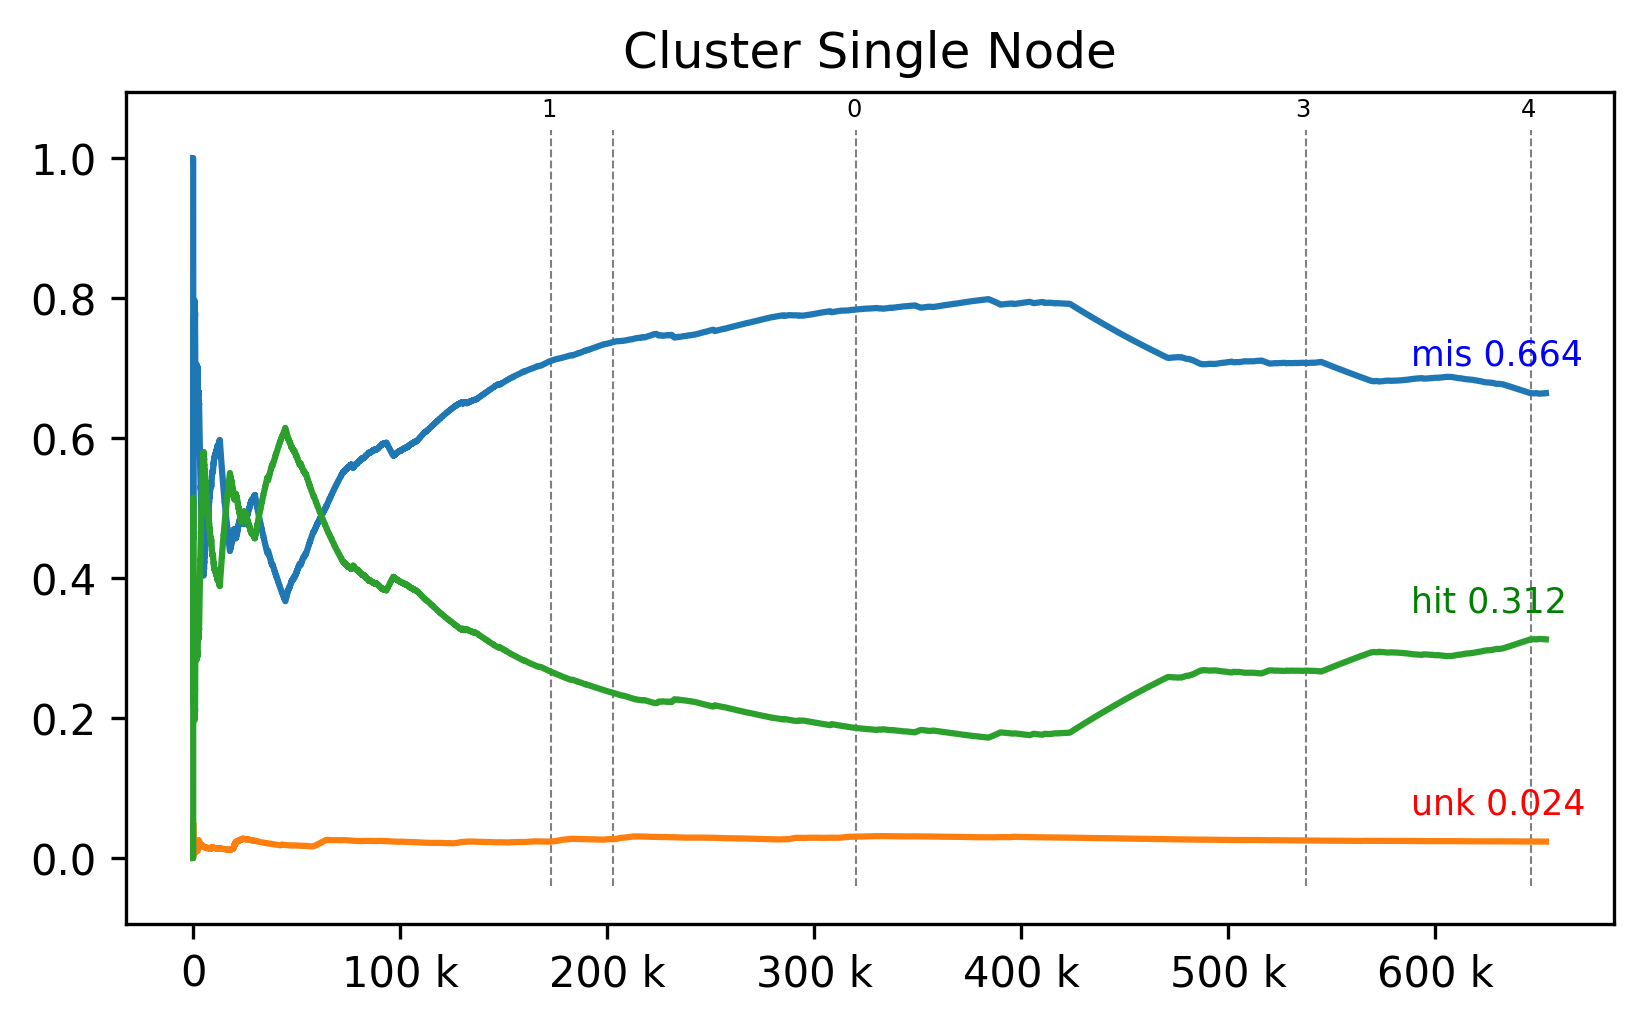
\includegraphics[width=1\linewidth]{experiments/tmi-base-log.png}
      \caption{Experimento \expC, \mfog com 1 nó e 4 núcleos.}
      \label{fig:single-flow}
    \end{subfigure}
    \hfill
    \begin{subfigure}{0.49\textwidth}
      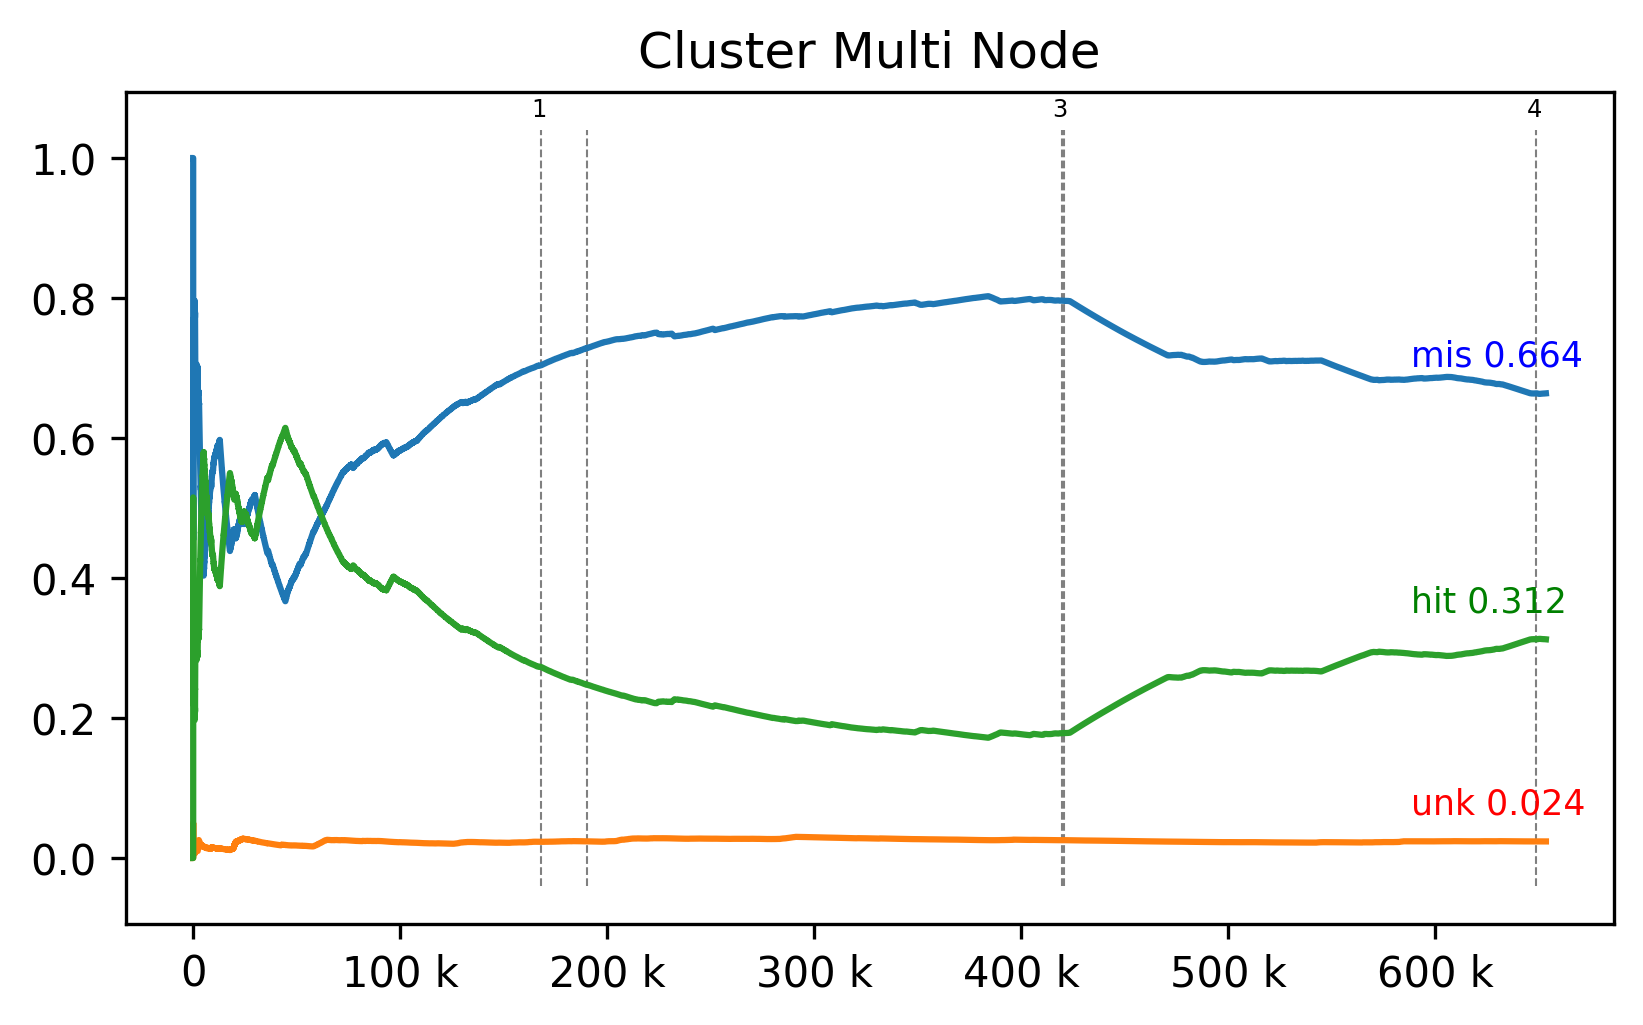
\includegraphics[width=1\linewidth]{experiments/tmi-n12-log.png}
      \caption{Experimento \expD, \mfog com 3 nós de 4 núcleos cada.}
      \label{fig:multi-flow}
    \end{subfigure}
    \caption{Visualização de fluxo do conjunto \emph{Kyoto} Dez. 2015.}
  \end{figure}
\end{frame}

\begin{frame}[fragile]{Resultados - Experimentos Adicionais}
  \begin{figure}
    \centering
    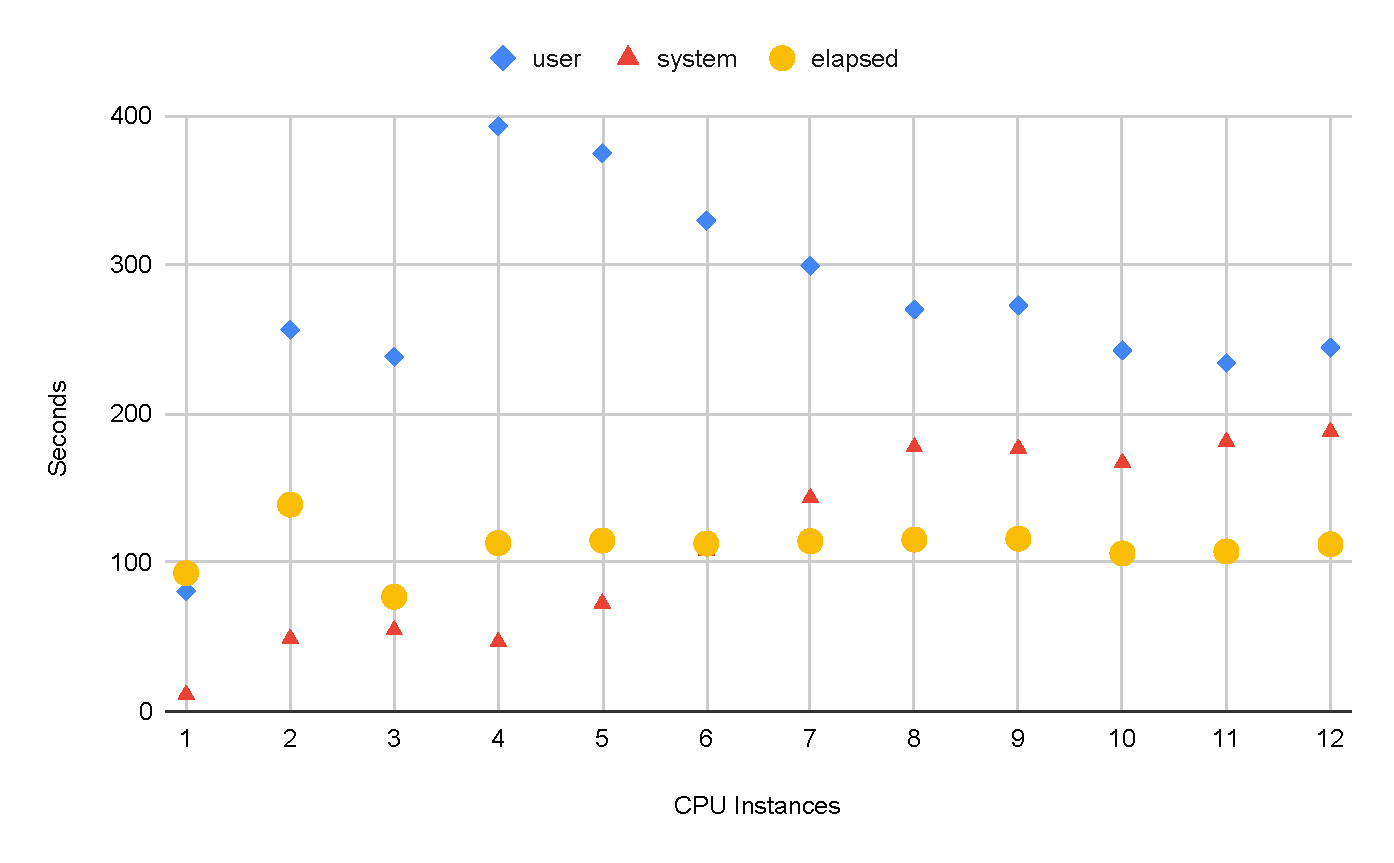
\includegraphics[width=0.7\linewidth,page=1]{experiments/speedup-clean.pdf}
    \caption{Métricas de tempo para execuções do \mfog com variação no número de processadores.}
    \label{fig:speedup}
  \end{figure}
\end{frame}

\begin{frame}{Resultados - Experimentos Adicionais}
    \begin{figure}[h]
      \centering
      \begin{subfigure}{0.49\textwidth}
        \centering
        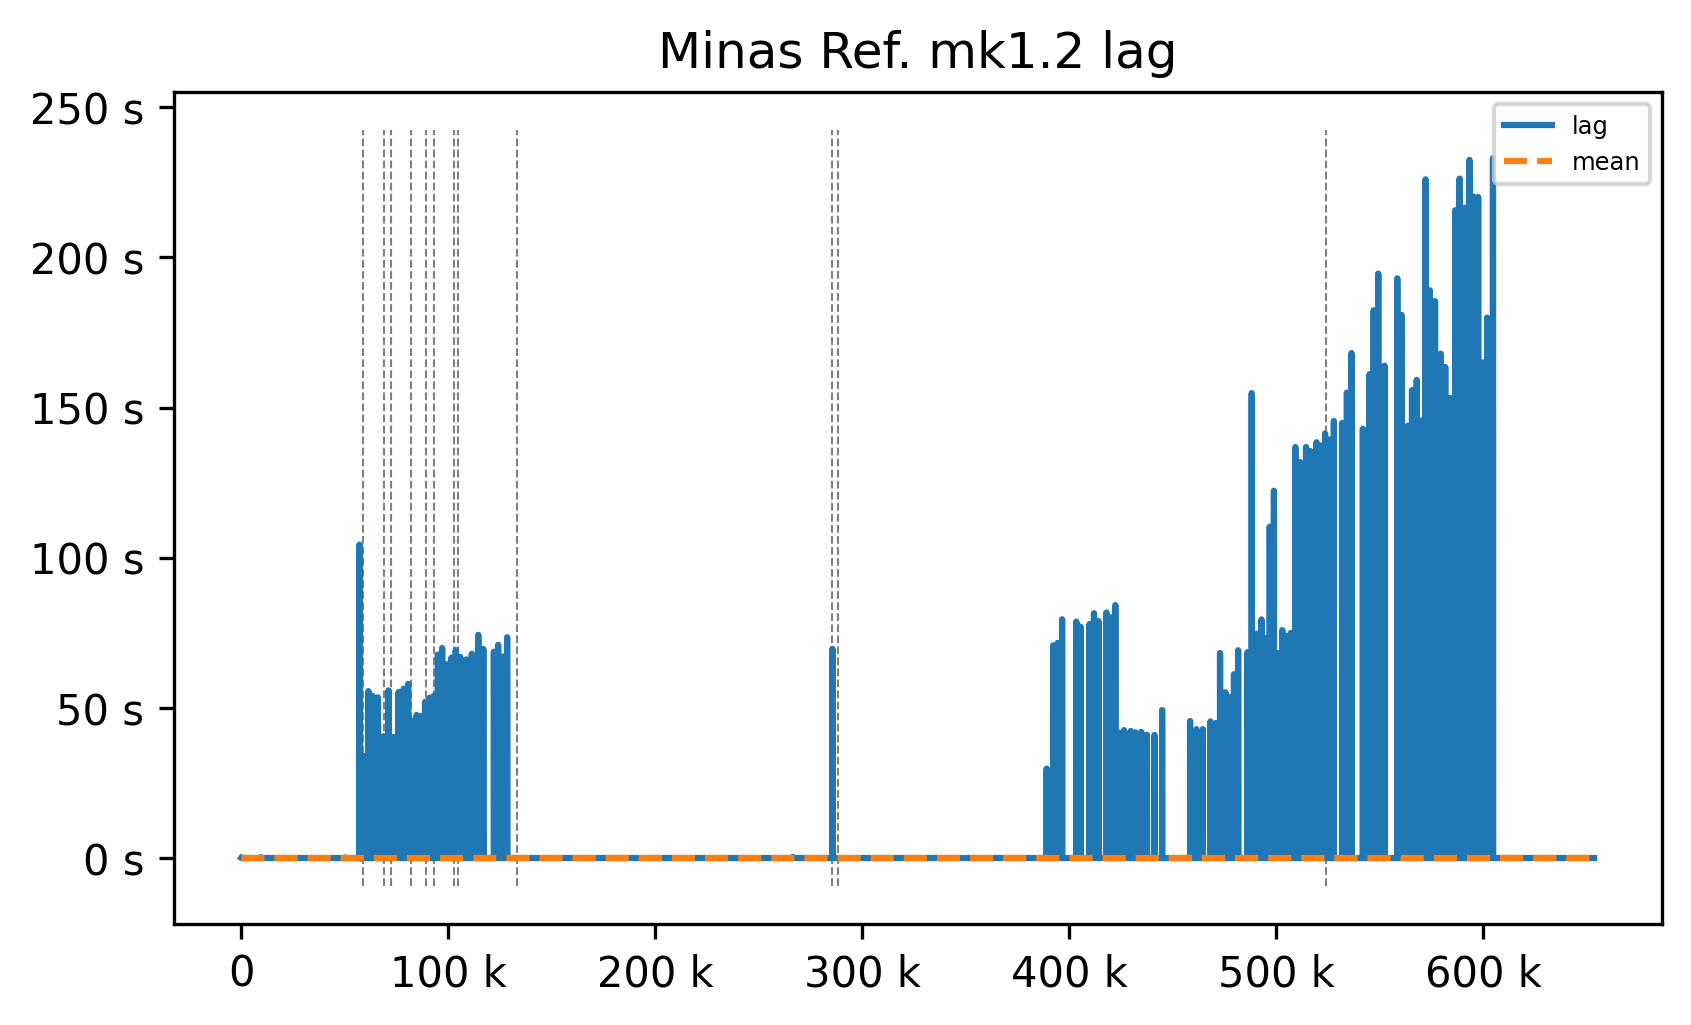
\includegraphics[width=1\linewidth]{experiments/lag-java.png}
        \caption{Implementação de referência.}
        \label{fig:lag-java}
      \end{subfigure}
      \hfill
      \begin{subfigure}{0.49\textwidth}
        \centering
        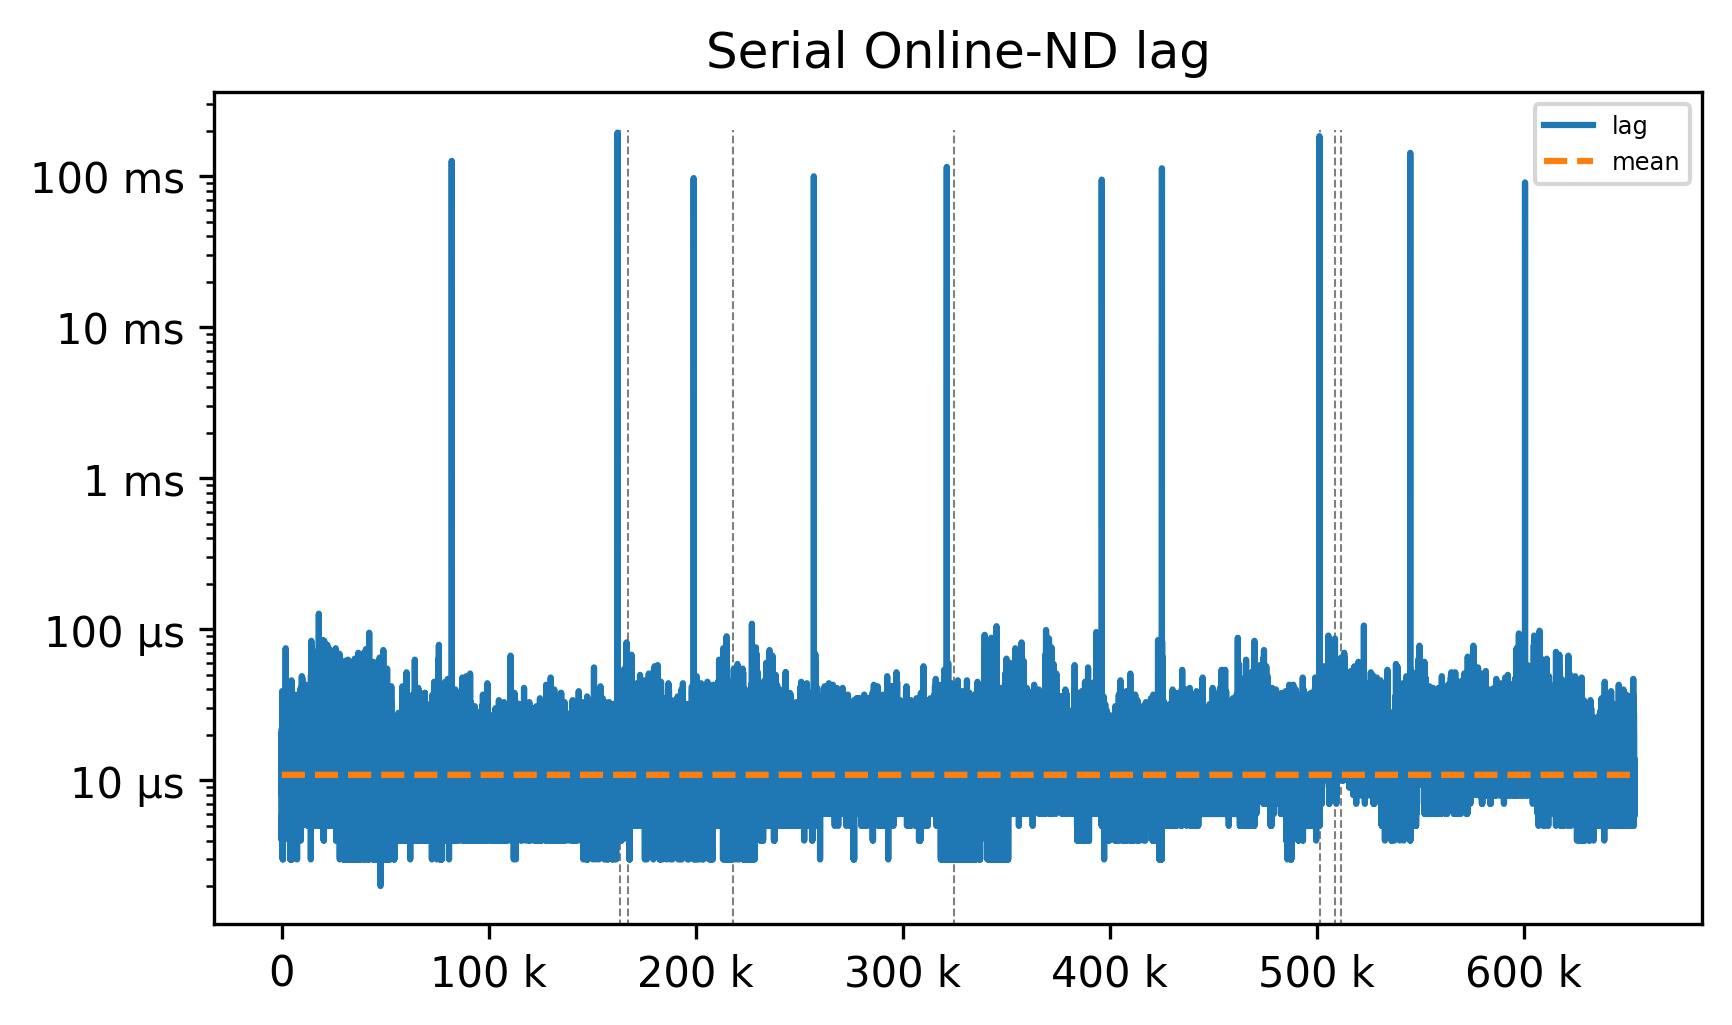
\includegraphics[width=1\linewidth]{experiments/lag-serial.png}
        \caption{Implementação sequencial.}
        \label{fig:lag-serial}
      \end{subfigure}
      \caption{Visualização de Latência das implementações de referência, sequencial
      e paralela do algoritmo \minas.}
      \label{fig:lag}
    \end{figure}
\end{frame}
\begin{frame}{Resultados - Experimentos Adicionais}
    \begin{figure}[h]
      \centering
      \begin{subfigure}{0.49\textwidth}
        \centering
        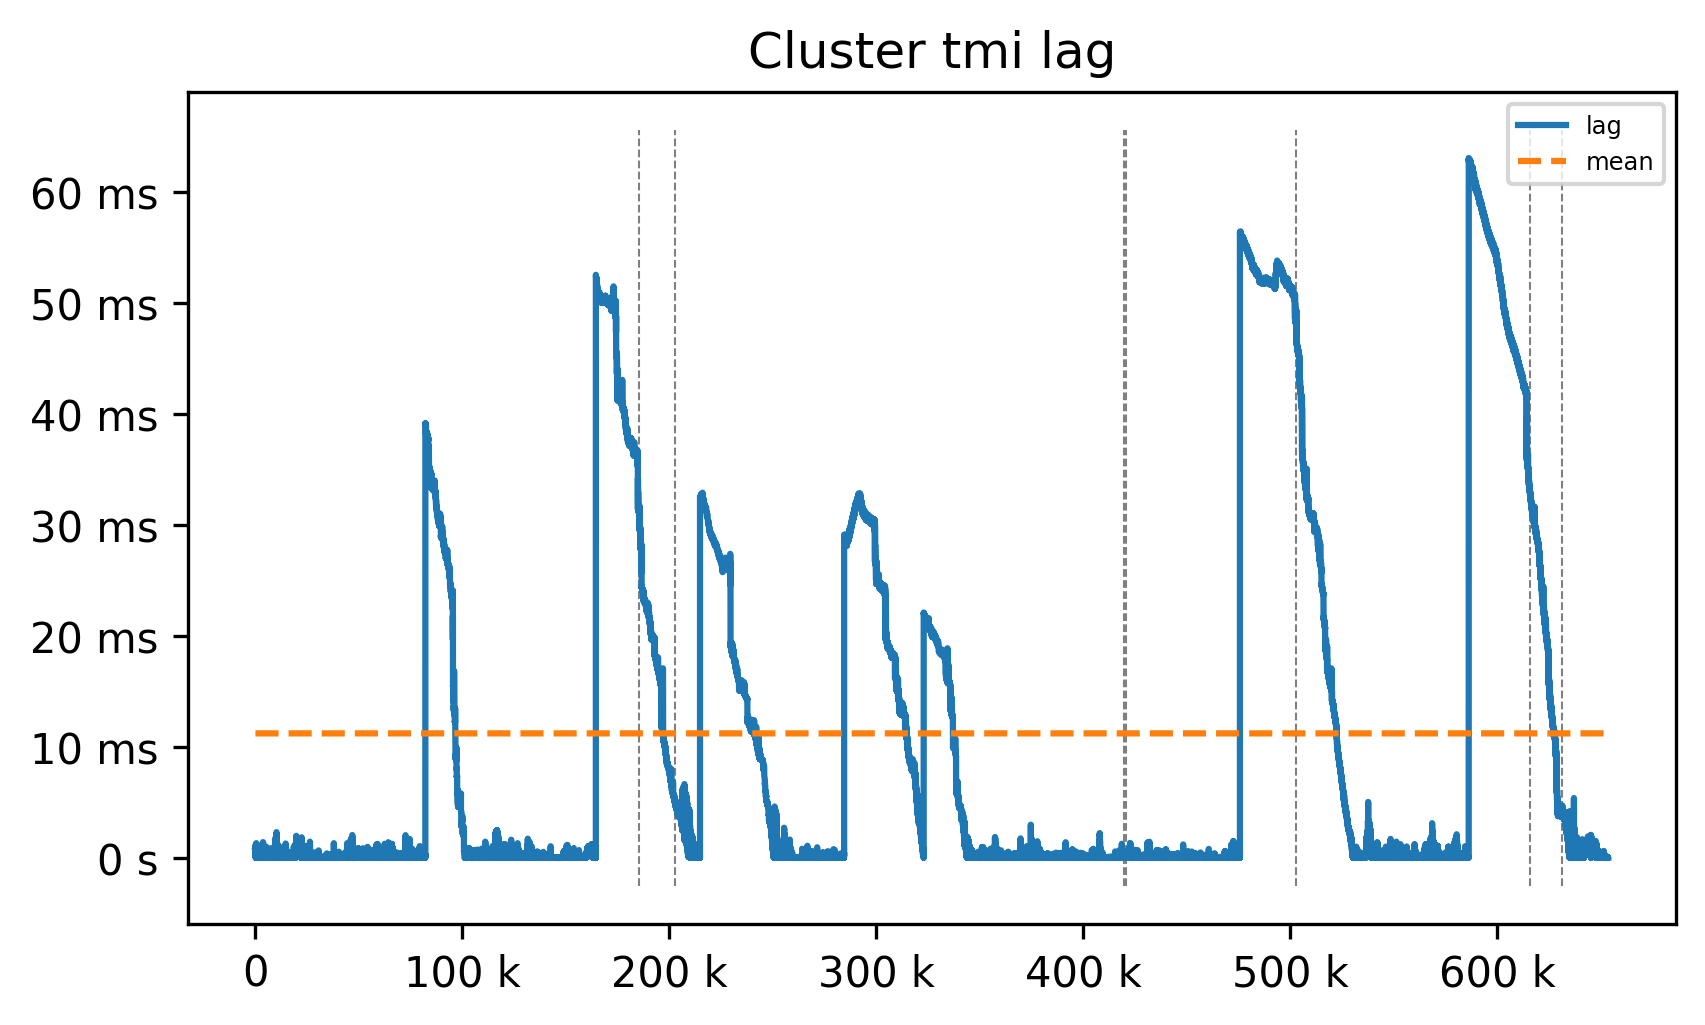
\includegraphics[width=1\linewidth]{experiments/lag-mfog.png}
        \caption{Implementação paralela.}
        \label{fig:lag-mfog}
      \end{subfigure}
      \caption{Visualização de Latência das implementações de referência, sequencial
      e paralela do algoritmo \minas.}
      \label{fig:lag-2}
    \end{figure}
\end{frame}

\section{Conclusão}
\begin{frame}{Conclusão}
  \begin{itemize}
    \item \mfog funciona;
    \item Distribuição tem efeito mas não é tão drástico;
    \item Não escala pelo CCR e eficiência;
    \item Trabalhos futuros:
    \begin{itemize}
      \item Outros algoritmos de agrupamento (CluStream);
      \item Estratégia de otimização da comunicação (micro ou mini batching);
      \item Explorar distribuição espacial dos clusters (polígonos sem
      sobreposição, árvore de busca);
      \item Algoritmo com modelo de tamanho fixo (máxima precisão com recursos disponíveis);
      \item Modelos com propriedade de conjuntos aditivos para sincronização
      entre redes distintas.
    \end{itemize}
  \end{itemize}
\end{frame}

\begin{frame}{Contribuições e Publicações}
  \begin{itemize}
    \item ICCSA 2021 \cite{Puhl2021};
    \item GitHub;
  \end{itemize}
\end{frame}

{\setbeamercolor{palette primary}{fg=black, bg=yellow}\begin{frame}[standout]
  Obrigado!
\end{frame}}

\begin{frame}[allowframebreaks]{Referências}
  \bibliography{99.referencias.bib}
\end{frame}

\appendix

\begin{frame}[fragile]{Extra}
  \begin{figure}[ht]
    \centering
    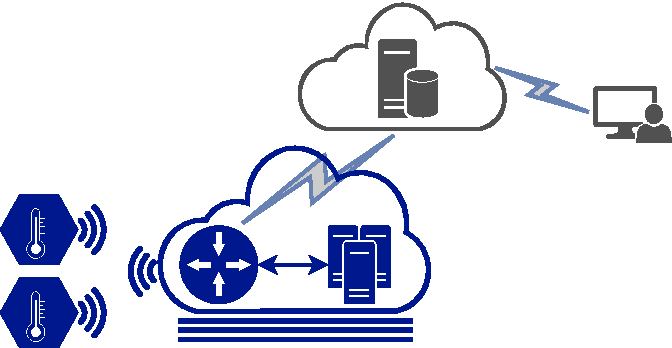
\includegraphics[width=0.8\textwidth]{figures/mfog-arch-fisica.svg.pdf}
    \caption{Arquitetura IoT tradicional.}
    \label{fig:ids-iot-phy}
  \end{figure}
\end{frame}

\end{document}
